\section{Buffer overflow}

Binary formats contain vital information regarding the file's organization on disk, memory loading procedures, file type (executable or library), machine class, and sections such as data and code. 

\paragraph*{ELF binaries}
ELF (Executable and Linkable Format) binaries adhere to the following structure:
\begin{itemize}
    \item \textit{ELF header}: this component delineates the overarching structure of the binary. 
        It specifies the file type and demarcates the boundaries for section and program headers.
    \item \textit{Program headers}: these headers elucidate how the file will be loaded into memory. 
        They segment the data into distinct segments and establish mappings between sections and segments.
    \item \textit{Section headers}: these headers provide a representation of the binary as it exists on disk. 
        They define various sections including:
        \begin{itemize}
            \item \texttt{.init}: contains executable instructions responsible for initializing the process.
            \item \texttt{.text}: holds the executable instructions of the program.
            \item \texttt{.bss}: reserved for statically-allocated variables, i.e., uninitialized data.
            \item \texttt{.data}: reserved for initialized data.
        \end{itemize}
\end{itemize}

\begin{definition}[\textit{Segment}]
    Segments represent the runtime view of an ELF (Executable and Linkable Format) binary. 
\end{definition}
They define how the binary will be loaded into memory, dividing the data into distinct segments and specifying the mapping between sections and segments. 
Segments play a crucial role in the execution of the program by providing the necessary information for the operating system to allocate memory and execute the binary.
\begin{definition}[\textit{Section}]
    Sections in an ELF binary contain linking and relocation information.
\end{definition}
They provide granular details about the various components of the binary, such as code, data, and symbols. 
Sections are essential for the linking process, aiding in resolving external symbols and determining memory layout. 
They also facilitate relocation, enabling the binary to be loaded and executed correctly in different memory locations. 
Sections serve as the building blocks for the organization and structure of the ELF binary.

\subsection{Process creation in Linux}
\paragraph*{Program creation}
When a program is executed, it undergoes a series of steps to be mapped into memory and organized for execution:
\begin{enumerate}
    \item \textit{Creation of virtual address space}: the kernel initiates by creating a virtual address space dedicated to the program's execution.
        This virtual address space provides isolation and abstraction, allowing each program to have its own memory layout.
    \item \textit{Loading information from executable file}: the kernel, with the assistance of the dynamic linker, loads relevant information from the executable file into the newly allocated address space. 
        This process involves loading the segments specified by the program headers of the ELF binary. 
        These segments typically include sections such as code, data, and other resources required for execution.
    \item \textit{Setup of stack and heap}: after loading the necessary information, the kernel sets up the stack and heap within the program's address space. 
        The stack is used for managing function calls and local variables, while the heap is utilized for dynamically allocated memory. 
        Additionally, the kernel determines the entry point of the program, where execution should begin, and directs control flow accordingly.
        Subsequently, the kernel initiates execution by jumping to the designated entry point of the program.
\end{enumerate}
\begin{figure}[H]
    \centering
    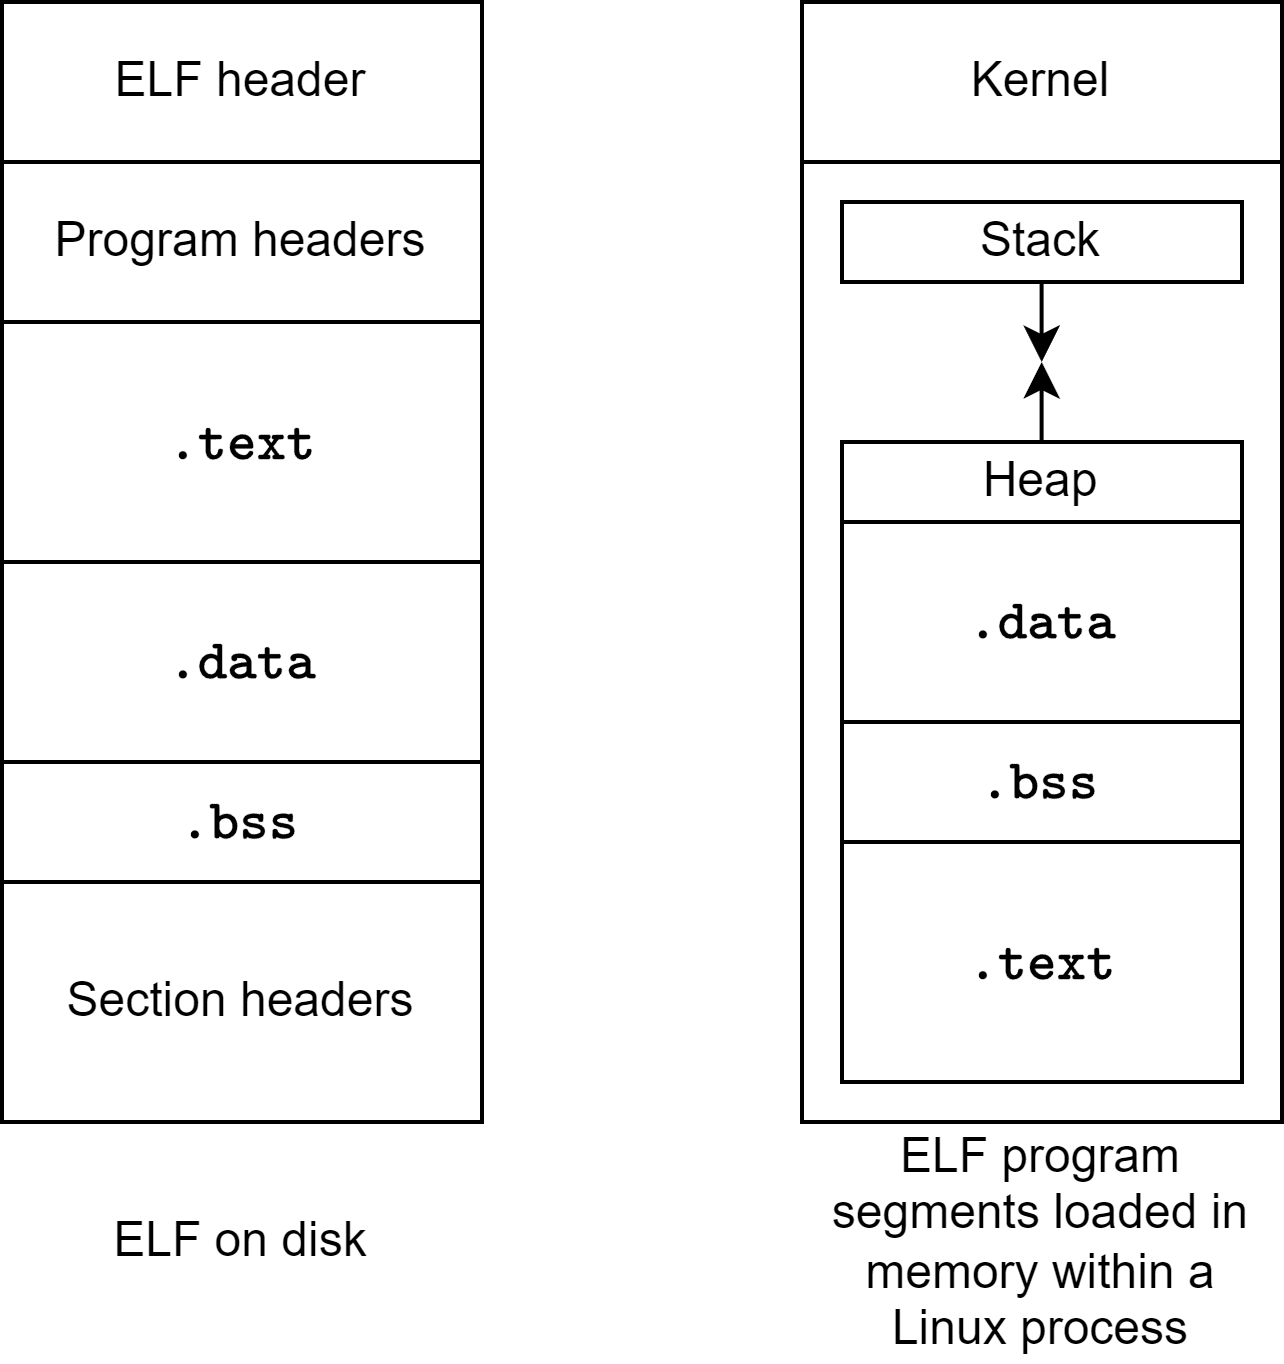
\includegraphics[width=0.6\linewidth]{images/linux.png}
    \caption{Process layout in Linux}
\end{figure}

\paragraph*{Program running}
When a program is correctly created, the virtual address space contains the following elements:
\begin{itemize}
    \item \textit{Argc, Env pointer, and stack}: This region encompasses statically allocated local variables, including environment variables, and function activation records. 
        The stack grows downward, towards lower addresses, as more function calls and local variables are added.
    \item \textit{Unallocated memory}.
    \item \textit{Heap}: dynamically allocated data resides in this section. 
        The heap grows upward, towards higher addresses, as more memory is dynamically allocated during program execution.
    \item \texttt{.data}: initialized data, such as global variables, is stored here.
    \item \texttt{.bss}: this section contains uninitialized data, which is zeroed out when the program begins execution.
    \item \texttt{.text}: the executable code, comprising machine instructions, resides in this segment.
    \item \textit{Shared libraries}. 
\end{itemize}
\begin{figure}[H]
    \centering
    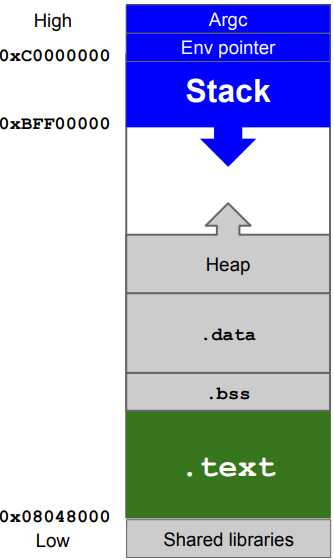
\includegraphics[width=0.6\linewidth]{images/stack.png}
    \caption{Code structure}
\end{figure}

\paragraph*{Program termination}
When the CPU is about to call the \texttt{foo()} function and \texttt{foo()} completes its execution, the CPU needs to determine where to jump next. 
Typically, after a function finishes executing, the control flow returns to the point in the program from which the function was called. 
This return address is crucial for maintaining the program's execution flow.

To achieve this, the CPU saves the current instruction pointer (EIP) onto the stack before jumping to the \texttt{foo()} function. 
When \texttt{foo()} completes its execution, the CPU retrieves the return address from the stack and jumps to that address, resuming execution from the point where the function was initially called.

This process ensures that the program maintains proper control flow and continues executing subsequent instructions after the completion of the \texttt{foo()} function.

\paragraph*{Summary}
When a function is called, its activation record, containing local variables, parameters, and the return address, is allocated on the stack. 
Control is transferred to the called function, and execution begins from its entry point.

When a function ends, it returns control to the original function caller by jumping back to the return address stored in its activation record. 
To ensure proper control flow, the CPU saves the return address of the caller's frame on the stack before jumping to the callee. 
Once the callee's execution is complete, the CPU retrieves the return address from the stack, restoring the caller's frame and continuing execution from where it left off.

Modern compilers typically employ a 16-byte ($2^4$) stack-boundary alignment by default for performance reasons, especially on certain CPUs.

When compiling with gcc without specifying \texttt{-mpreferred-stack-boundary=2} ($2^2$, or 4 bytes), the resulting code will allocate memory in increments of 16 bytes, even for smaller data types.
This means that, for variables or data types smaller than 16 bytes, additional padding will be added to maintain the 16-byte alignment.
This alignment strategy optimizes memory access and improves performance, particularly for CPU architectures that benefit from aligned memory access patterns.

\subsection{Stack smashing}
Stack smashing, a term first mentioned in a 1972 report (ESD-TR-7315), gained widespread attention and was popularized by the 1994 article ``Smashing the Stack for Fun and Profit'' by Aleph1, which is considered a must-read in the field of computer security.

The concept of stack smashing often occurs in C programming due to unsafe practices. 
For example, consider a function \texttt{foo()} that allocates a buffer, such as \texttt{char buf[8]}, without performing proper size checking. 
If this buffer is subsequently filled with data that exceeds its allocated size, it can lead to a buffer overflow vulnerability.

Several standard C library functions are prone to causing stack smashing if not used carefully. 
These include: \texttt{strcpy}, \texttt{strcat}, \texttt{fgets}, \texttt{gets}, \texttt{sprintf}, \texttt{scanf}.

Failure to properly handle these functions can result in stack smashing vulnerabilities, which attackers may exploit to execute arbitrary code, crash the program, or gain unauthorized access to sensitive information. 
Therefore, it's essential for programmers to be vigilant and use safer alternatives or apply proper input validation and buffer size checks to mitigate the risk of stack smashing vulnerabilities in their code.

Instead of going out of the stack space we need to jump to a valid memory
location that contains, or can be filled with,
valid executable machine code. 
Possible solutions are: 
\begin{itemize}
    \item Environment variable.
    \item Built-in, existing functions.
    \item Memory that we can control: the buffer itself or some other variable.
\end{itemize}

\subsection{Buffer address guessing}
Guessing the buffer address for executing arbitrary machine code in the overflowed buffer can be challenging due to several factors:
\begin{itemize}
    \item \textit{Proximity to ESP}: one common approach is to guess that the overflowed buffer is located somewhere near the stack pointer (ESP). 
        Debugging tools like GDB (GNU Debugger) can help in determining the approximate location of ESP at runtime.
    \item \textit{Variability}: unfortunately, the exact address of the buffer may change with each execution or across different machines. 
        This variability makes it difficult to reliably predict the buffer's address.
    \item \textit{CPU precision}: CPUs are not intelligent enough to handle imprecise memory accesses gracefully. 
        Even a small offset error can lead to failure in fetching and executing instructions, potentially causing the program to crash or exhibit unexpected behavior.
\end{itemize}
The problem of precision arises because executing arbitrary machine code relies on accurately predicting the memory location of the buffer. 
However, due to the dynamic nature of memory allocation and the lack of precision in CPU operations, achieving reliable execution of arbitrary code in a stack overflow scenario is challenging.
Security measures such as Address Space Layout Randomization (ASLR) further complicate this task by introducing additional randomness to memory addresses, making it even harder to predict the location of the buffer.

In practical scenarios, obtaining the ESP (stack pointer) value can be achieved by using a debugger or reading from the process directly. 
However, it's important to note that certain debuggers, like gdb, may introduce an offset to the allocated process memory. 
Consequently, the ESP value obtained from gdb (first case) might differ by a few words from the ESP value obtained by reading directly within the process (second case).

Despite these methods, a precision issue persists. 
Even with accurate ESP values, there's still a challenge in precisely determining the location of the buffer. 
This lack of precision can impede the reliable execution of arbitrary code in a stack overflow scenario. 
Further solutions to address this precision problem will be discussed in the subsequent slides.

\paragraph*{NOP sled}
To locate the desired address within the buffer, we can utilize a NOP sled. 
A NOP sled is essentially a sequence of No Operation instructions, represented by the hexadecimal value 0x90 on x86 architecture.
These instructions do nothing when executed, serving as a landing strip for the program's execution flow.
The idea is that wherever the program falls within the NOP sled range, it will encounter valid instructions, and eventually reach the end of the sled where the actual executable code resides.

At the beginning of the buffer, we place a sequence of NOP instructions, creating the NOP sled. 
This sled acts as a safe landing zone for the program's execution flow.
By jumping to anywhere within the NOP sled range, we ensure that even if the precise location of the buffer is not accurately determined, the program will still land on valid instructions within the NOP sled and continue execution until it reaches the desired executable code.

In essence, the NOP sled provides a flexible and reliable mechanism for redirecting the program's execution flow to the intended code, overcoming the precision issues associated with predicting the exact memory address of the buffer.

\subsection{Process to run}
Historically, the primary goal of an attacker has been to spawn a privileged shell, either on a local or remote machine.
\begin{definition}[\textit{Shell code}]
    Shell code refers to a sequence of machine instructions necessary to open a shell, typically a privileged one.
\end{definition}
In essence, shell code can perform a wide range of actions, not limited to spawning a shell. 
However, spawning a shell has been a common objective due to the elevated privileges it provides.

The desired process for an attacker typically involves invoking the \texttt{execve} system call. 
This system call executes a program referred to by its pathname. 
\texttt{execve} is part of a family of system calls required to execute privileged instructions.

\paragraph*{Calling convention}
In Linux systems, invoking a system call involves executing a software interrupt using the \texttt{int} instruction, passing the value \texttt{0x80}. 
This triggers the kernel to execute the specified system call, such as \texttt{execve}, and perform the requested action: 
\begin{enumerate}
    \item \texttt{movl \$syscall\_number, eax}
    \item Syscall arguments GP registers (ebc, ecx, edx): 
        \begin{enumerate}
            \item \texttt{mov arg1, \%ebx}
            \item \texttt{mov arg2, \%ecx}
            \item \texttt{mov arg3, \%edx}
        \end{enumerate}
    \item \texttt{int 0x80} 
    \item Syscall is executed.
\end{enumerate}

\paragraph*{Shell code}
Creating shell code involves a process that typically starts with high-level code and involves translating it into machine instructions, often using assembly language. However, an alternative approach is to write the code in C and then extract the relevant instructions to compose the shell code. The process can be outlined as follows:
\begin{enumerate}
    \item \textit{Write high-level code}: begin by writing the desired functionality in high-level C code.
    \item \textit{Compile and disassembly}: compile the C code and then disassemble the resulting binary to obtain its assembly instructions.
    \item \textit{Analyze assembly}: analyze the disassembled code to identify and extract only the relevant instructions needed to achieve the desired functionality. 
        This often involves cleaning up the code and removing unnecessary instructions.
    \item \textit{Extract opcode}: identify the opcode (operation code) for each relevant instruction. The opcode represents the specific operation to be performed by the CPU.
    \item \textit{Create the shell code}: finally, assemble the extracted opcodes into a sequence of bytes to form the shell code. 
        This shell code can be injected into a vulnerable program or used in exploits to achieve the desired outcome.
\end{enumerate}

\paragraph*{Alternative}
We demonstrated this capability using an overflowed buffer, but it can also be achieved with other memory regions.
The benefit is the ability to execute this remotely (where input equals code). 
However, there are drawbacks: the buffer may not be sufficiently large, the memory must be designated as executable, and reliable address guessing is necessary.

\subsection{Defending against buffer overflows}
We can apply a layered defense strategy against buffer overflows: 
\begin{enumerate}
    \item \textit{Source code level defenses}: identify and eliminate vulnerabilities within the source code.
    \item \textit{Compiler level defenses}: render vulnerabilities non-exploitable through compiler-level techniques.
    \item \textit{Operating system level defenses}: implement measures on the operating system level to obstruct attacks, or at the very least increase their difficulty.
\end{enumerate}

\paragraph*{Source code level defenses}
C/C++ programming can be fortified to prevent buffer overflows, with an understanding that such overflows stem from programmer errors. 
This necessitates educating developers, integrating security measures into the System Development Life Cycle, conducting targeted testing, and employing source code analyzers.
Moreover, the adoption of safer libraries can contribute significantly. 
For instance, utilizing functions from the Standard Library like \texttt{strncpy} and \texttt{strncat}, which allow specifying the length parameter explicitly, or opting for BSD versions such as \texttt{strlcpy} and \texttt{strlcat}.
Furthermore, languages featuring dynamic memory management, such as Java, inherently offer greater resilience against these vulnerabilities.
Integrating such languages into the development process can serve as an additional layer of defense.

\paragraph*{Compiler level defenses}
Warnings issued during compile time serve as an initial line of defense, alerting developers to potential vulnerabilities before execution.
Additionally, randomized reordering of stack variables, while considered a temporary measure, can introduce variability, making it harder for attackers to exploit memory vulnerabilities.
Moreover, embedding stack protection mechanisms during compilation enhances security.
The canary mechanism, for instance, involves inserting a sentinel value between local variables and control values. 
During the function's epilogue, the integrity of this canary is verified. If tampering is detected upon function return, the program is terminated.
There are various types of canaries implemented for enhancing security:
\begin{itemize}
    \item Terminator canaries are constructed using terminator characters, often /0, which cannot be copied by string-copy functions. 
        This characteristic prevents them from being overwritten during potential attacks.
    \item Random canaries are generated as random sequences of bytes when the program is executed. 
        This randomness adds an additional layer of defense against buffer overflow attacks. 
        They are commonly implemented using options like \texttt{-fstack-protector} in GCC.
    \item Random XOR canaries, similar to random canaries, are also randomly generated but are additionally XORed with a portion of the structure that requires protection. 
        This XOR operation adds complexity to the canary, making it more difficult for attackers to manipulate even in scenarios where buffer overflow doesn't occur.
\end{itemize}

\paragraph*{Operating system level defenses}
OS Level Defenses encompass several protective measures:
\begin{itemize}
    \item Non-executable stack configuration ensures that data is distinguished from executable code, mitigating the risk of stack smashing attacks on local variables. 
        However, it's worth noting that certain programs, such as older versions of the JVM, may require executing code on the stack, posing a challenge to this defense mechanism.
    \item To enforce non-executable stack policies, hardware mechanisms like the NX bit are leveraged. 
    \item Despite non-executable stack defenses, attackers may bypass them by redirecting the return address to existing machine instructions, a technique known as code-reuse attacks. 
        Common variants include return to libc (ret2libc) attacks using C library functions or more sophisticated methods like return-oriented programming (ROP).
    \item Address Space Layout Randomization (ASLR) further fortifies defenses by repositioning memory elements, including the stack, at random locations during each execution.
        This randomness makes it challenging for attackers to predict return addresses accurately. 
        ASLR is active by default in Linux kernels newer than 2.6.12, with a typical randomization range of 8MB, configurable through /proc/sys/kernel/randomize\_va\_space.
\end{itemize}